\documentclass[conference]{IEEEtran}
\IEEEoverridecommandlockouts
% The preceding line is only needed to identify funding in the first footnote. If that is unneeded, please comment it out.
\usepackage{cite}
\usepackage{amsmath,amssymb,amsfonts}
\usepackage{algorithmic}
\usepackage{graphicx}
\usepackage{textcomp}
\usepackage{xcolor}
\def\BibTeX{{\rm B\kern-.05em{\sc i\kern-.025em b}\kern-.08em
    T\kern-.1667em\lower.7ex\hbox{E}\kern-.125emX}}
\begin{document}

\title{Simple Action Model: Enabling LLM to Sequential Function Calling Tool Chain\\
}

\author{

% \and
\IEEEauthorblockN{Rajat Sandeep Sen}
\IEEEauthorblockA{\textit{ Department of AI\&DS} \\
\textit{SJCET Palai}\\
Kottayam, Kerala \\
rajatsandeepsen2025@ai.sjcetpalai.ac.in}

\\

\IEEEauthorblockN{Sharon Prashant Jose}
\IEEEauthorblockA{\textit{ Department of AI\&DS} \\
\textit{SJCET Palai}\\
Kottayam, Kerala \\
sharonprashantjose2025@ai.sjcetpalai.ac.in}

\and

\IEEEauthorblockN{Amalkrishna M} 
\IEEEauthorblockA{\textit{ Department of AI\&DS} \\
\textit{SJCET Palai}\\
Kottayam, Kerala \\
amalkrishna28032003@gmail.com}

\\

\IEEEauthorblockN{Neena Joseph}
\IEEEauthorblockA{\textit{ Department of AI\&DS} \\
\textit{SJCET Palai}\\
Kottayam, Kerala \\
nestofneena@gmail.com}

\and

\IEEEauthorblockN{Prithviraj R} 
\IEEEauthorblockA{\textit{ Department of AI\&DS} \\
\textit{SJCET Palai}\\
Kottayam, Kerala \\
prithvirajr0306@gmail.com}





% \and
}

\maketitle

\begin{abstract}
    Today, LLMs are everywhere. It is making human internet life a lot easier than ever. Every day new sophisticated models are released. But these models are not good enough to become personal assistants like the Jarvis from the Sci-fi movie IronMan. This paper proposes a way to enable any LLM to execute complex requirements in real-world applications. By leveraging state-of-the-art Large Language models, we can create a simple action model that can understand the environment around them. Eventually, these models can help or assist humans in real-time applications. The Sequential Function Calling Tool Chain System aims to bridge the gap between human language understanding and computer programming.
\end{abstract}

\begin{IEEEkeywords}
    Large language model, Action model, OpenAPI format, and Function Calling Tools
\end{IEEEkeywords}

\section{Introduction}
Nowadays, a world without AI is impossible to imagine. New models will come every day, and new architecture will improve its performance. Multi-modality or a Mixture of Models is not enough to become a personal assistant. Graph-based models take up a lot of computation in the case of complex function calling. Simple Question, ” What if the one good model with one request is enough to execute multiple functions sequentially?”.

The integration of OpenAPI schema with LLM can make a decent action model that can understand the API specs of that specific application. The large language model will take prompts and decide what to do. From the programming side, we’ll parse the information and execute it. A simple action model is done.

By implementing a custom JSON parser alongside an OpenAPI schema-type system it is possible to utilize one model as main decision making inside an application. This technology works faster compared to other solutions but requires a much more intelligent language model. 

This helps to provide stable and intelligent AI assistants in any applications that uphold the integrity and standards of API formats.This research paper also leads to the exploration of Multiple and Sequential Function calling toolchain that utilizes a State-of-the-Art Language model to enhance the security, time efficiency, and flexibility of building AI applications. 

The purpose of this paper is to explore and improve existing solutions of function calling tools available in the open-source software community. This paper also aims to provide a new approach to prompting the LLMs without fine-tuning.

\section{Literature Survey}
These literature reviews provide knowledge about the existing research done by various scholars and open-source developers.

[1] Luyu Gao, Aman Madaan, Shuyan Zhou, Uri Alon, Pengfei Liu, Yiming
Yang, Jamie Callan, Graham Neubig, PAL: Program-aided
Language Models, Jan 2023, They had introduced a new architecture of LLMs wrapper that are trained on both interpreted programming language and natural languages. These system are utilized with ability to run code directly at runtime. [2] Tatsuro Inaba, Hirokazu Kiyomaru, Fei Cheng, Sadao Kurohash,
MultiTool-CoT: GPT-3 Can Use Multiple External Tools with Chain
of Thought Prompting (2023), They had introduced a new architecture of LLMs that can use multiple external tools with Chain of Thought Prompting. [3] Yujia Qin, Shihao Liang, Yining Ye, Kunlun Zhu, Lan Yan, Yaxi Lu,
Yankai Lin, Xin Cong, Xiangru Tang, Bill Qian, Sihan Zhao, Lauren
Hong, Runchu Tian, Ruobing Xie, Jie Zhou, Mark Gerstein, Dahai Li, Zhiyuan Liu, Maosong Sun, TOOLLLM: FACILITATING LARGE
LANGUAGE MODELS TO MASTER 16000+ REAL-WORLD APIS 2023, They had introduced a new architecture of LLMs that can master 16000+ real-world APIs. [4] Sehoon Kim, Suhong Moon, Ryan Tabrizi, Nicholas Lee, Michael W.
Mahoney, Kurt Keutzer, Amir Gholami An LLM Compiler
for Parallel Function Calling Jun 2024, They had introduced a new architecture of LLMs that can compile parallel function calling. 


\section{Methodology}
The approach of the Sequential Function calling tool is using the popular and newest OpenAPI schema 3.0. By fetching the schema JSON from the backend url is converted to a type parser like Zod (npm) at build time. The prompt captured from the user is fed to LLM with proper type annotation of OpenAPI schema. Any popular open-source model can be used to understand and extract object/JSON data from user's prompts. The extracted data are then loaded into a custom JSON parser that supports extra keywords from standard JSON format. The parser moves the data to OpenAPI client libraries like OpenAPI-Fetch (npm) which fetches results from the backend. The result is then passed to the next function in the chain. The process is repeated until the end of the chain. But LLM is used once just to write ”what to do in this environment” according to users prompts and type definition.

\subsection{Schema Preparation}\label{AA}
The preparation of the schema at build time utilizes popular libraries like OpenAPI-TS (npm) and OpenAPI-Zod (npm). It’ll generate types schema for use in few-shot learning of LLM and zod schema for parsing the input and return data to and from LLM. Feeding the LLM with raw OpenAPI schema is a waste of tokens and context window, that’s why it is a crucial step to create a simpler version of schema. This process involves collecting open API schema JSON (by fetching from the application backend server), parsing and preprocessing, and then structuring it in a way that is useful for teaching the language model. 

The recorded schema was obtained from backend frameworks that support swagger-ui or other libraries that generate OpenAPI. Simplified parser schema and type are written to a coding file (here typescript programming language is used) and saved into a folder. Later this obtained schema was resized to smaller chunks if the schema is larger than the model's context window. The graph-based structure is used to label and store nodes. This graph data structure will help to query through large schema faster in runtime.

\begin{figure}[htbp]
    \centering
    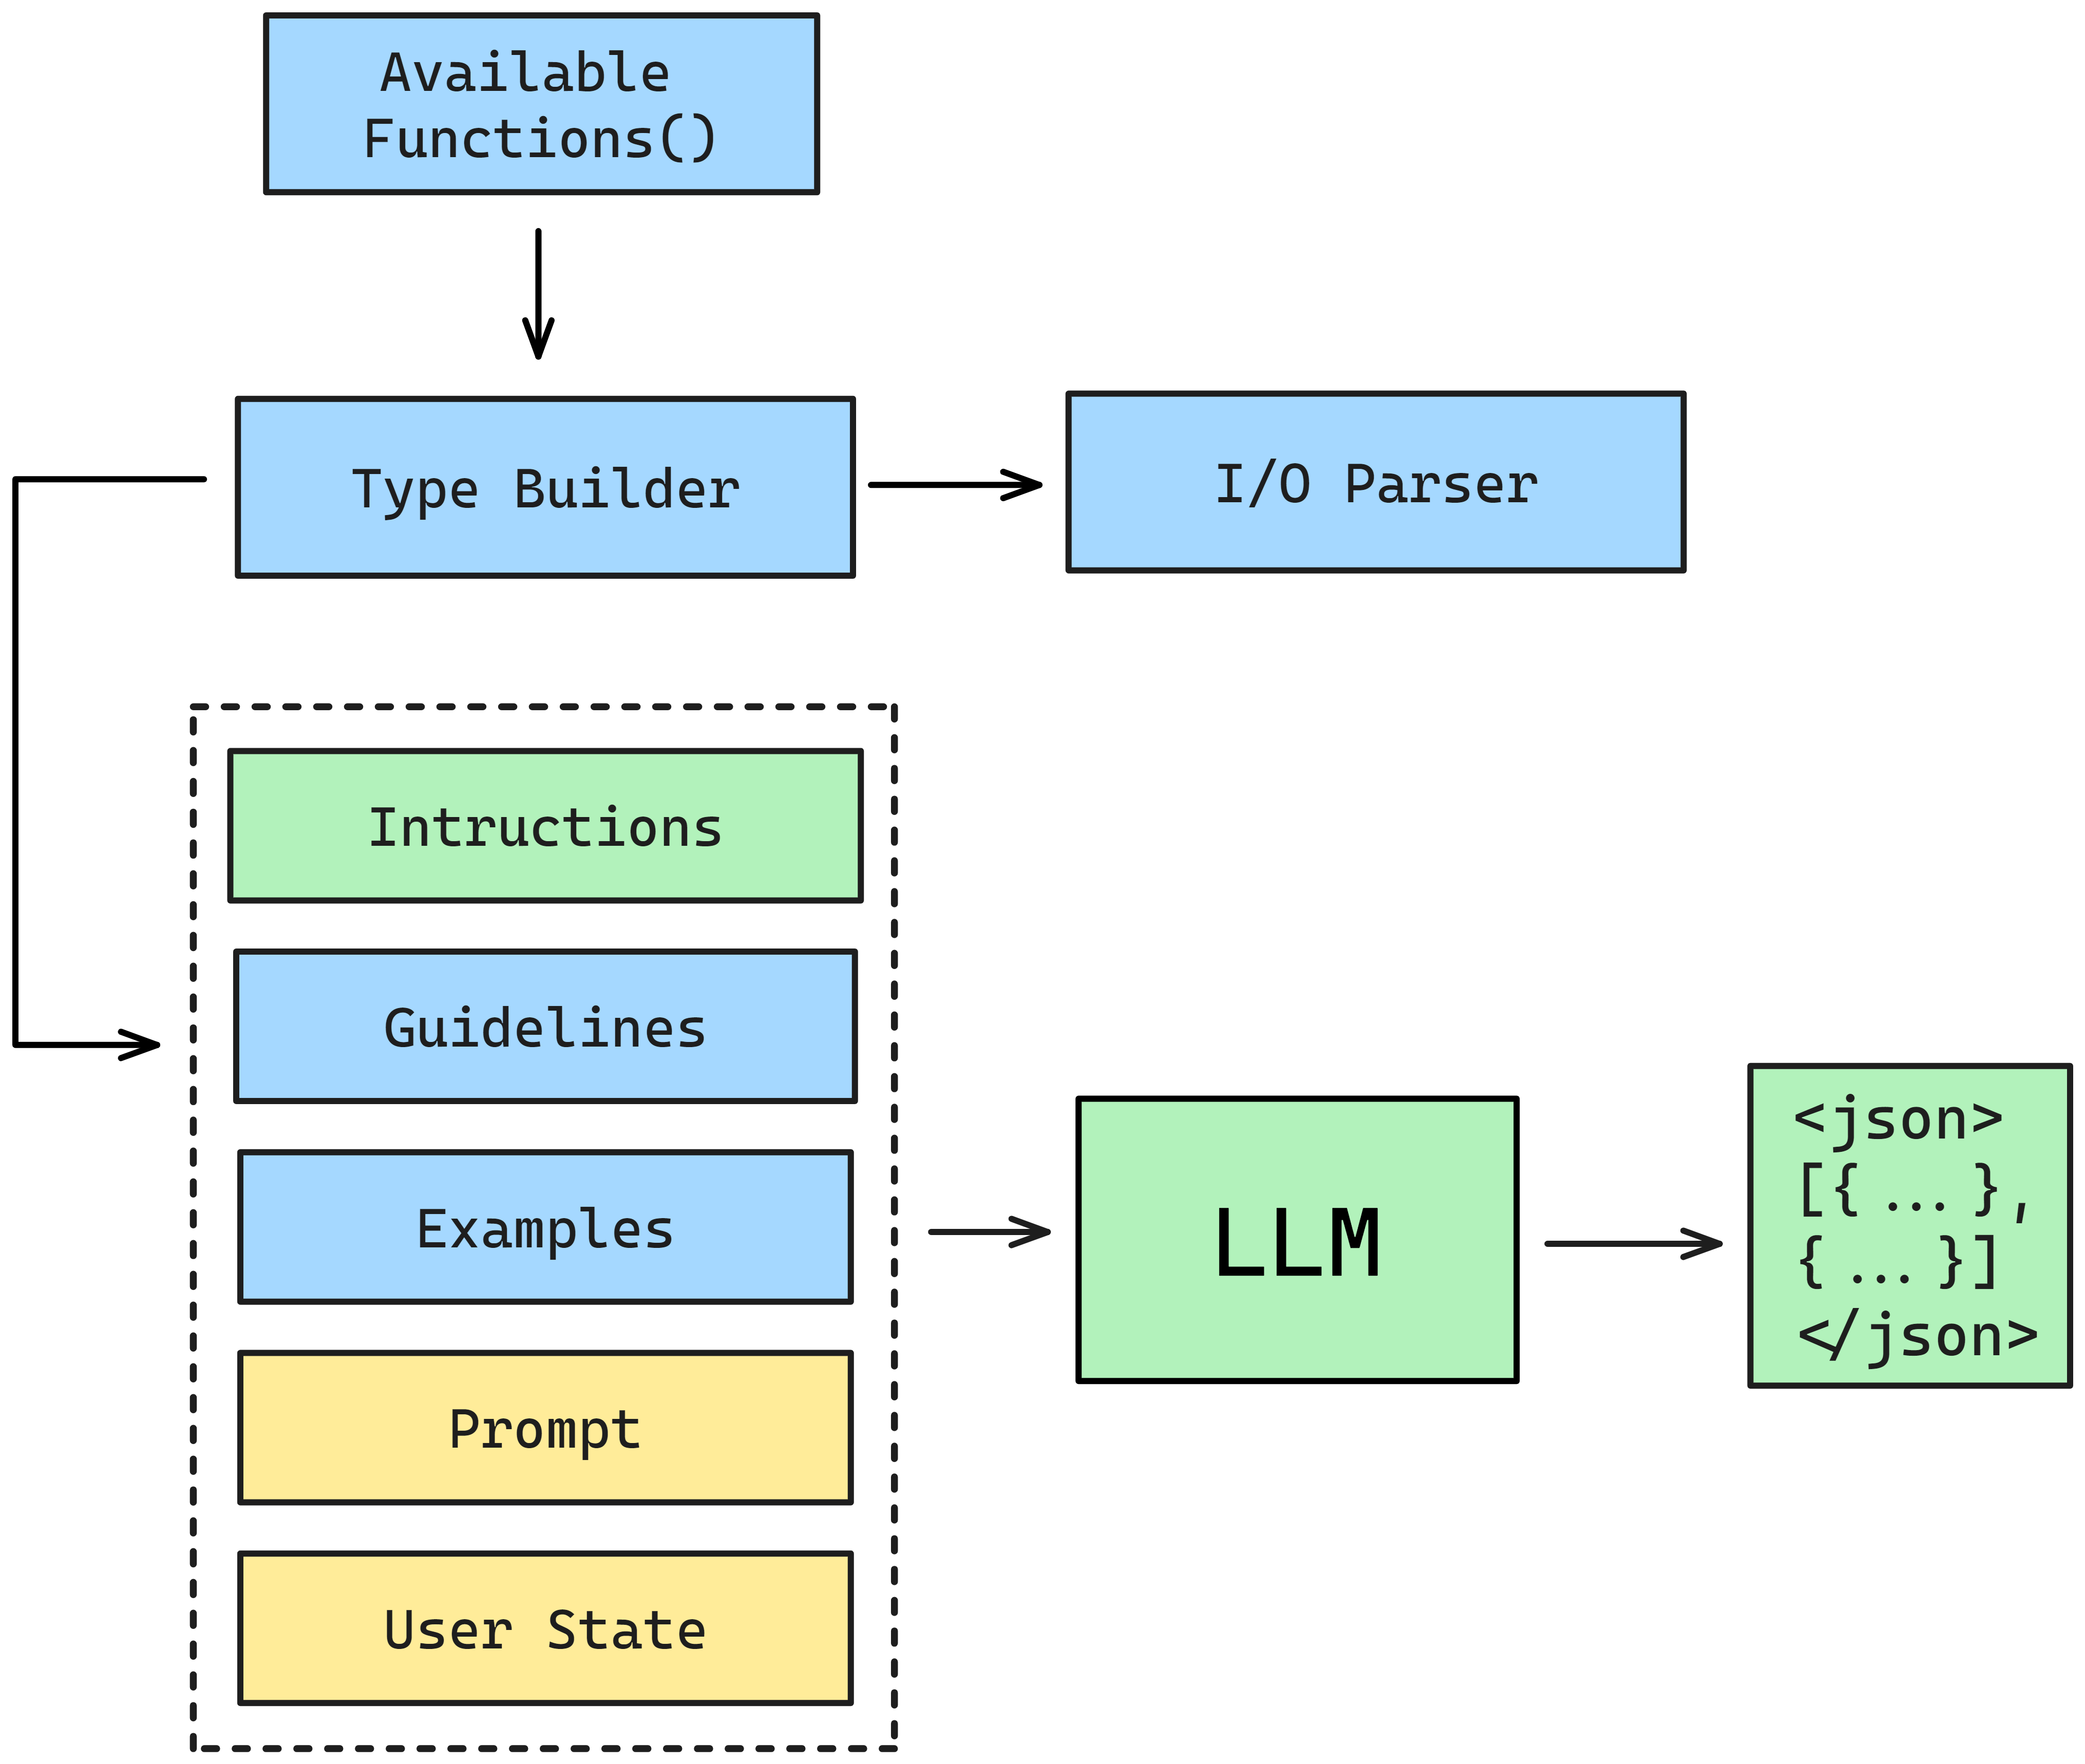
\includegraphics[width=0.48\textwidth]{images/without-finetuning.png}  
    \caption{Block Diagram for Normal In-context Learning}
    \label{fig}
\end{figure}

\subsection{Prompt Preparation}

The LLM is always instructed to return a response in JSON tags, making the data easier to extract from a string. Also, the available functions list (or schema from OpenAPI) is converted to easy, type definitions, which makes it easier to understand for the LLMs. 

But normally open source LLMs are stupid without examples. They are trained on general knowledge, and that's why a few shots of in-context learning are needed to make it understand the environment. 

Also, the fine-tuning approach is great if the type definition and instructions are larger than the context window of the LLM used. Teach the Model with the entire OpenAPI schema and examples before deploying to production gives better results in response and saves a lot of tokens while prompting each time

\begin{figure}[htbp]
\centering
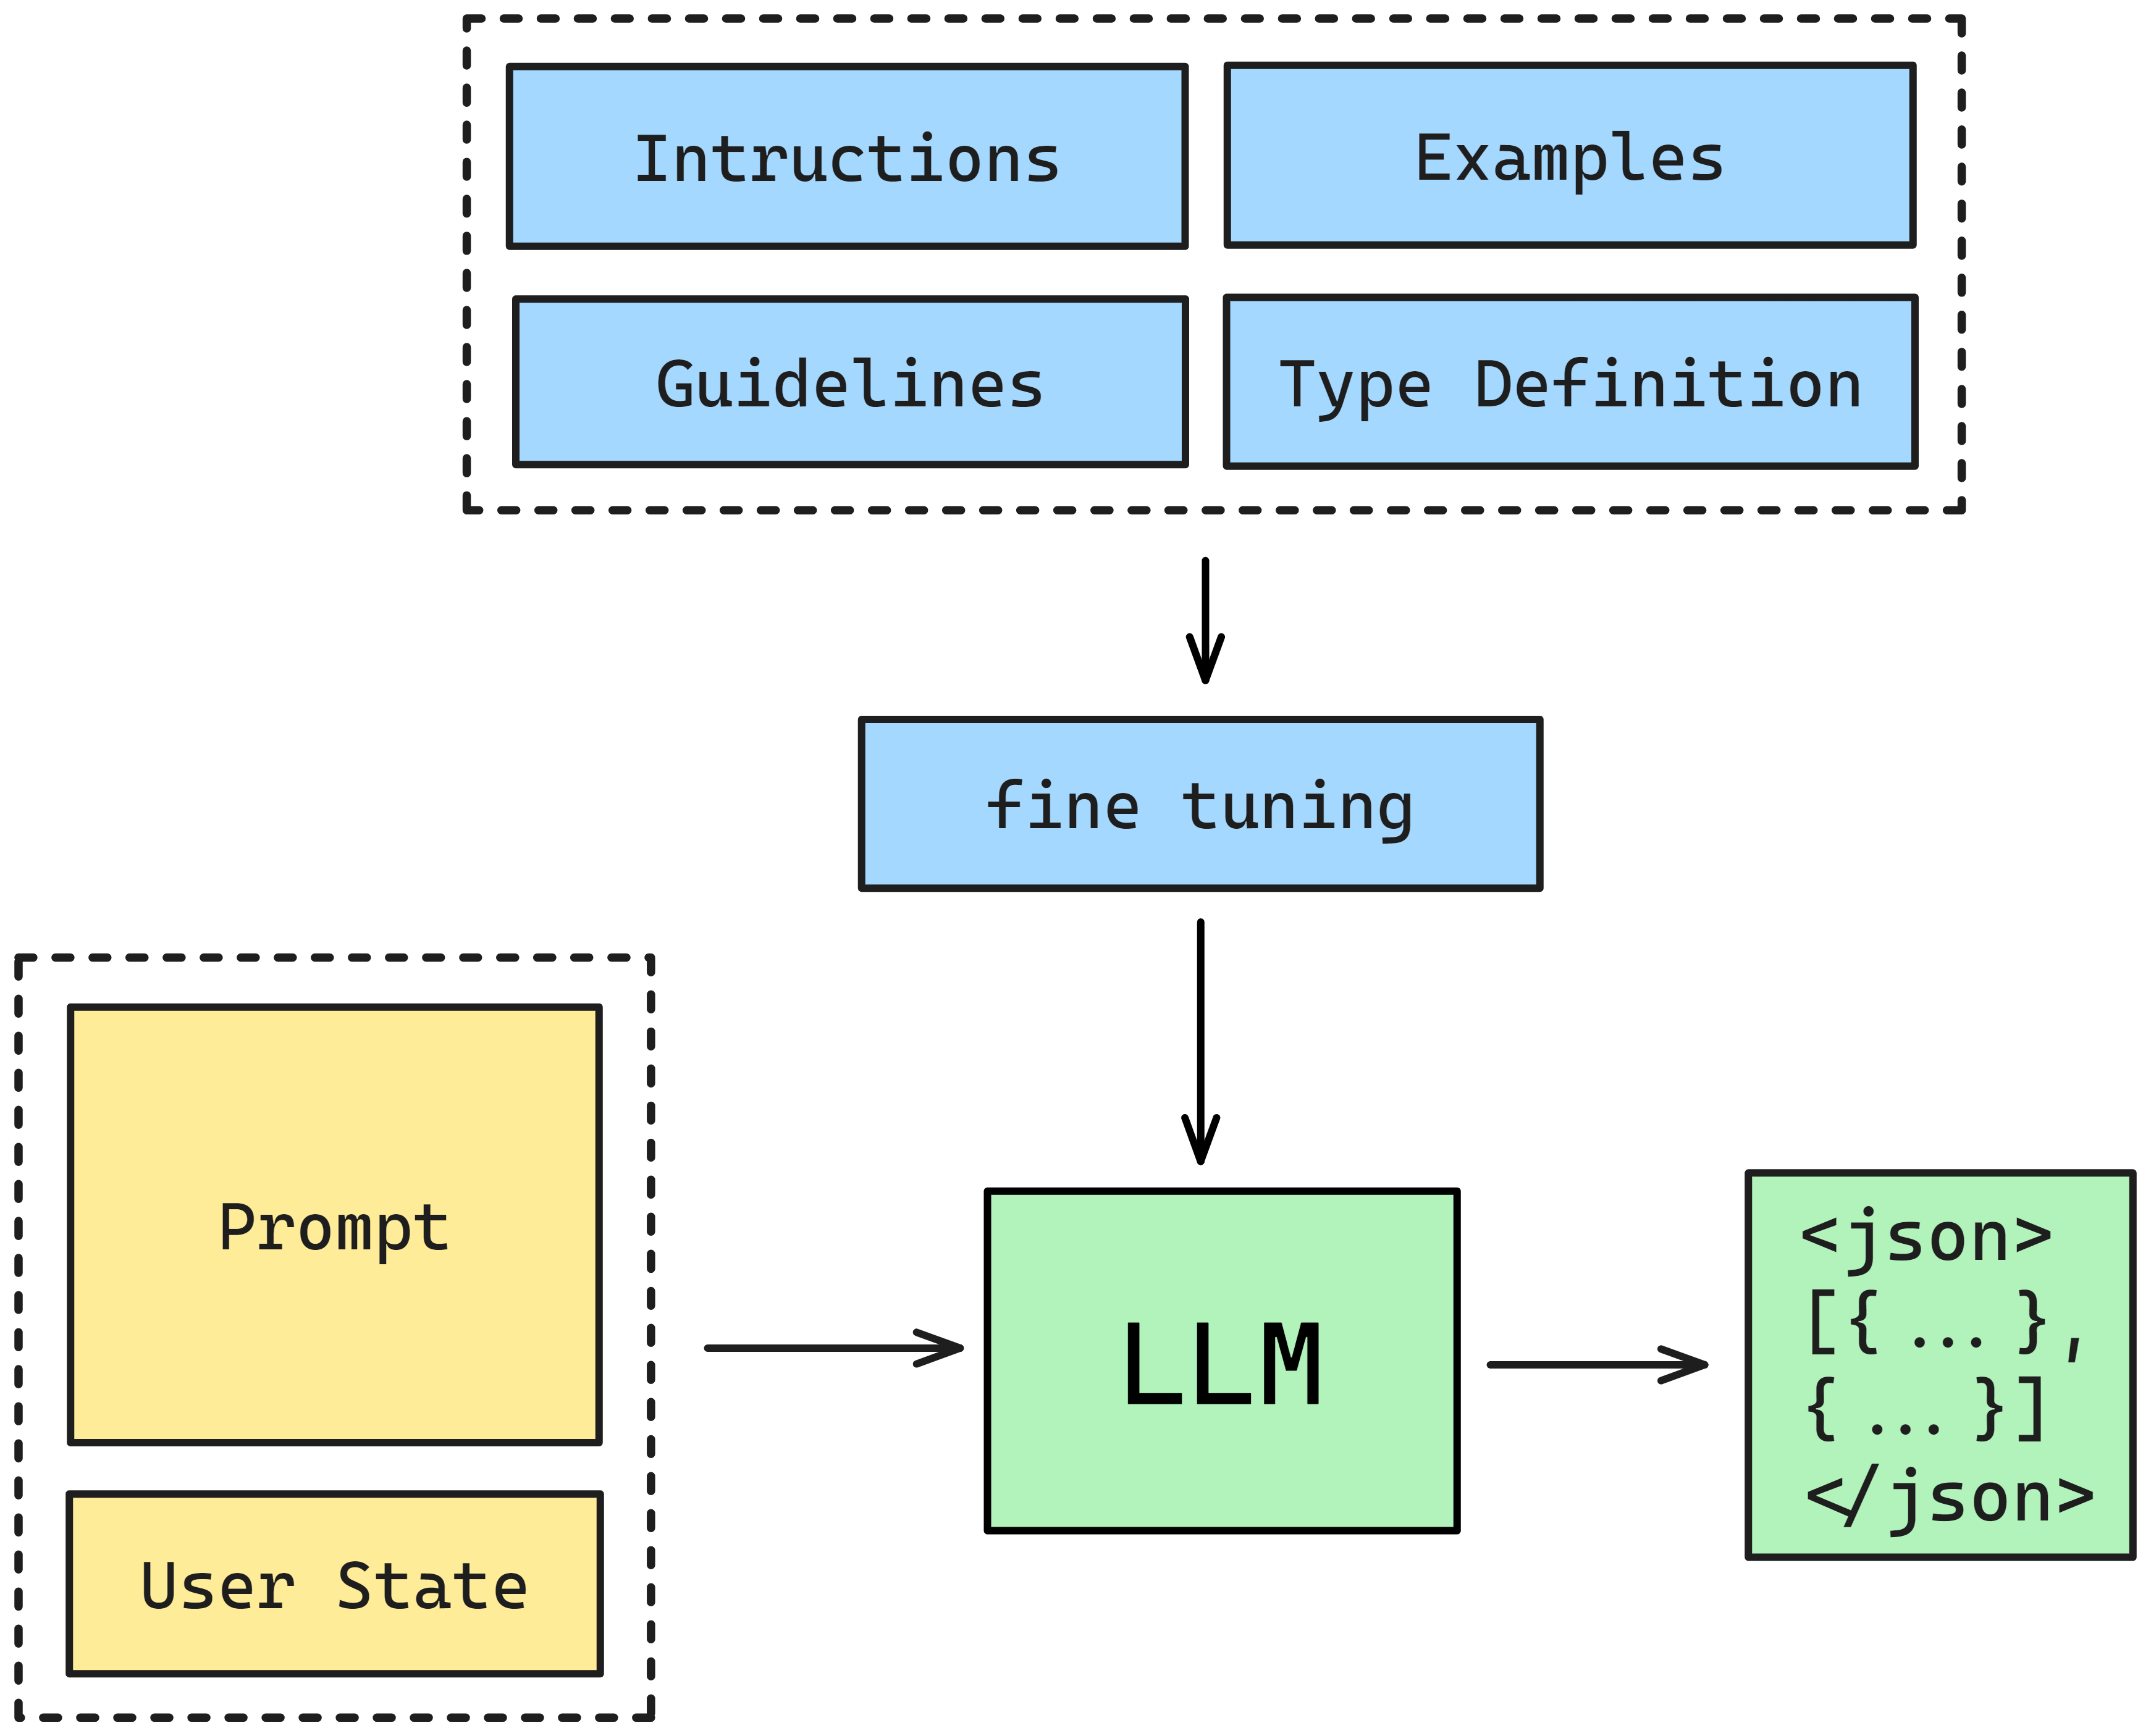
\includegraphics[width=0.48\textwidth]{images/fine-tuned.png}  
\caption{Block Diagram for Fine tuned learning}
\label{fig}
\end{figure}

\subsection{Server Architecture}
Initially, the developer specifies the backend URL and OpenAPI schema URL in the configuration file. Fetches the schema from the backend applications and prepares the schema at build time. The server is a standalone backend that listens to end-user prompts. The server takes the user prompt, types the definition of the OpenAPI schema, and sends it to LLM. The developer also needs to mention the provider and model in the configuration file. Then the LLM returns with some JSON data wrapped with JSON tag. The data shows ”what to run”, ”where to fetch” and ”what are the parameter and request body”. Then parses the JSON data and sends it to the Action engine. The engine takes care of function calling and chaining. Finally, the result is sent back to the user in JSON format (or stream the UI if the server is built with meta-frameworks like Next.js or Nuxt.js).

\begin{figure}[htbp]
    \centering
    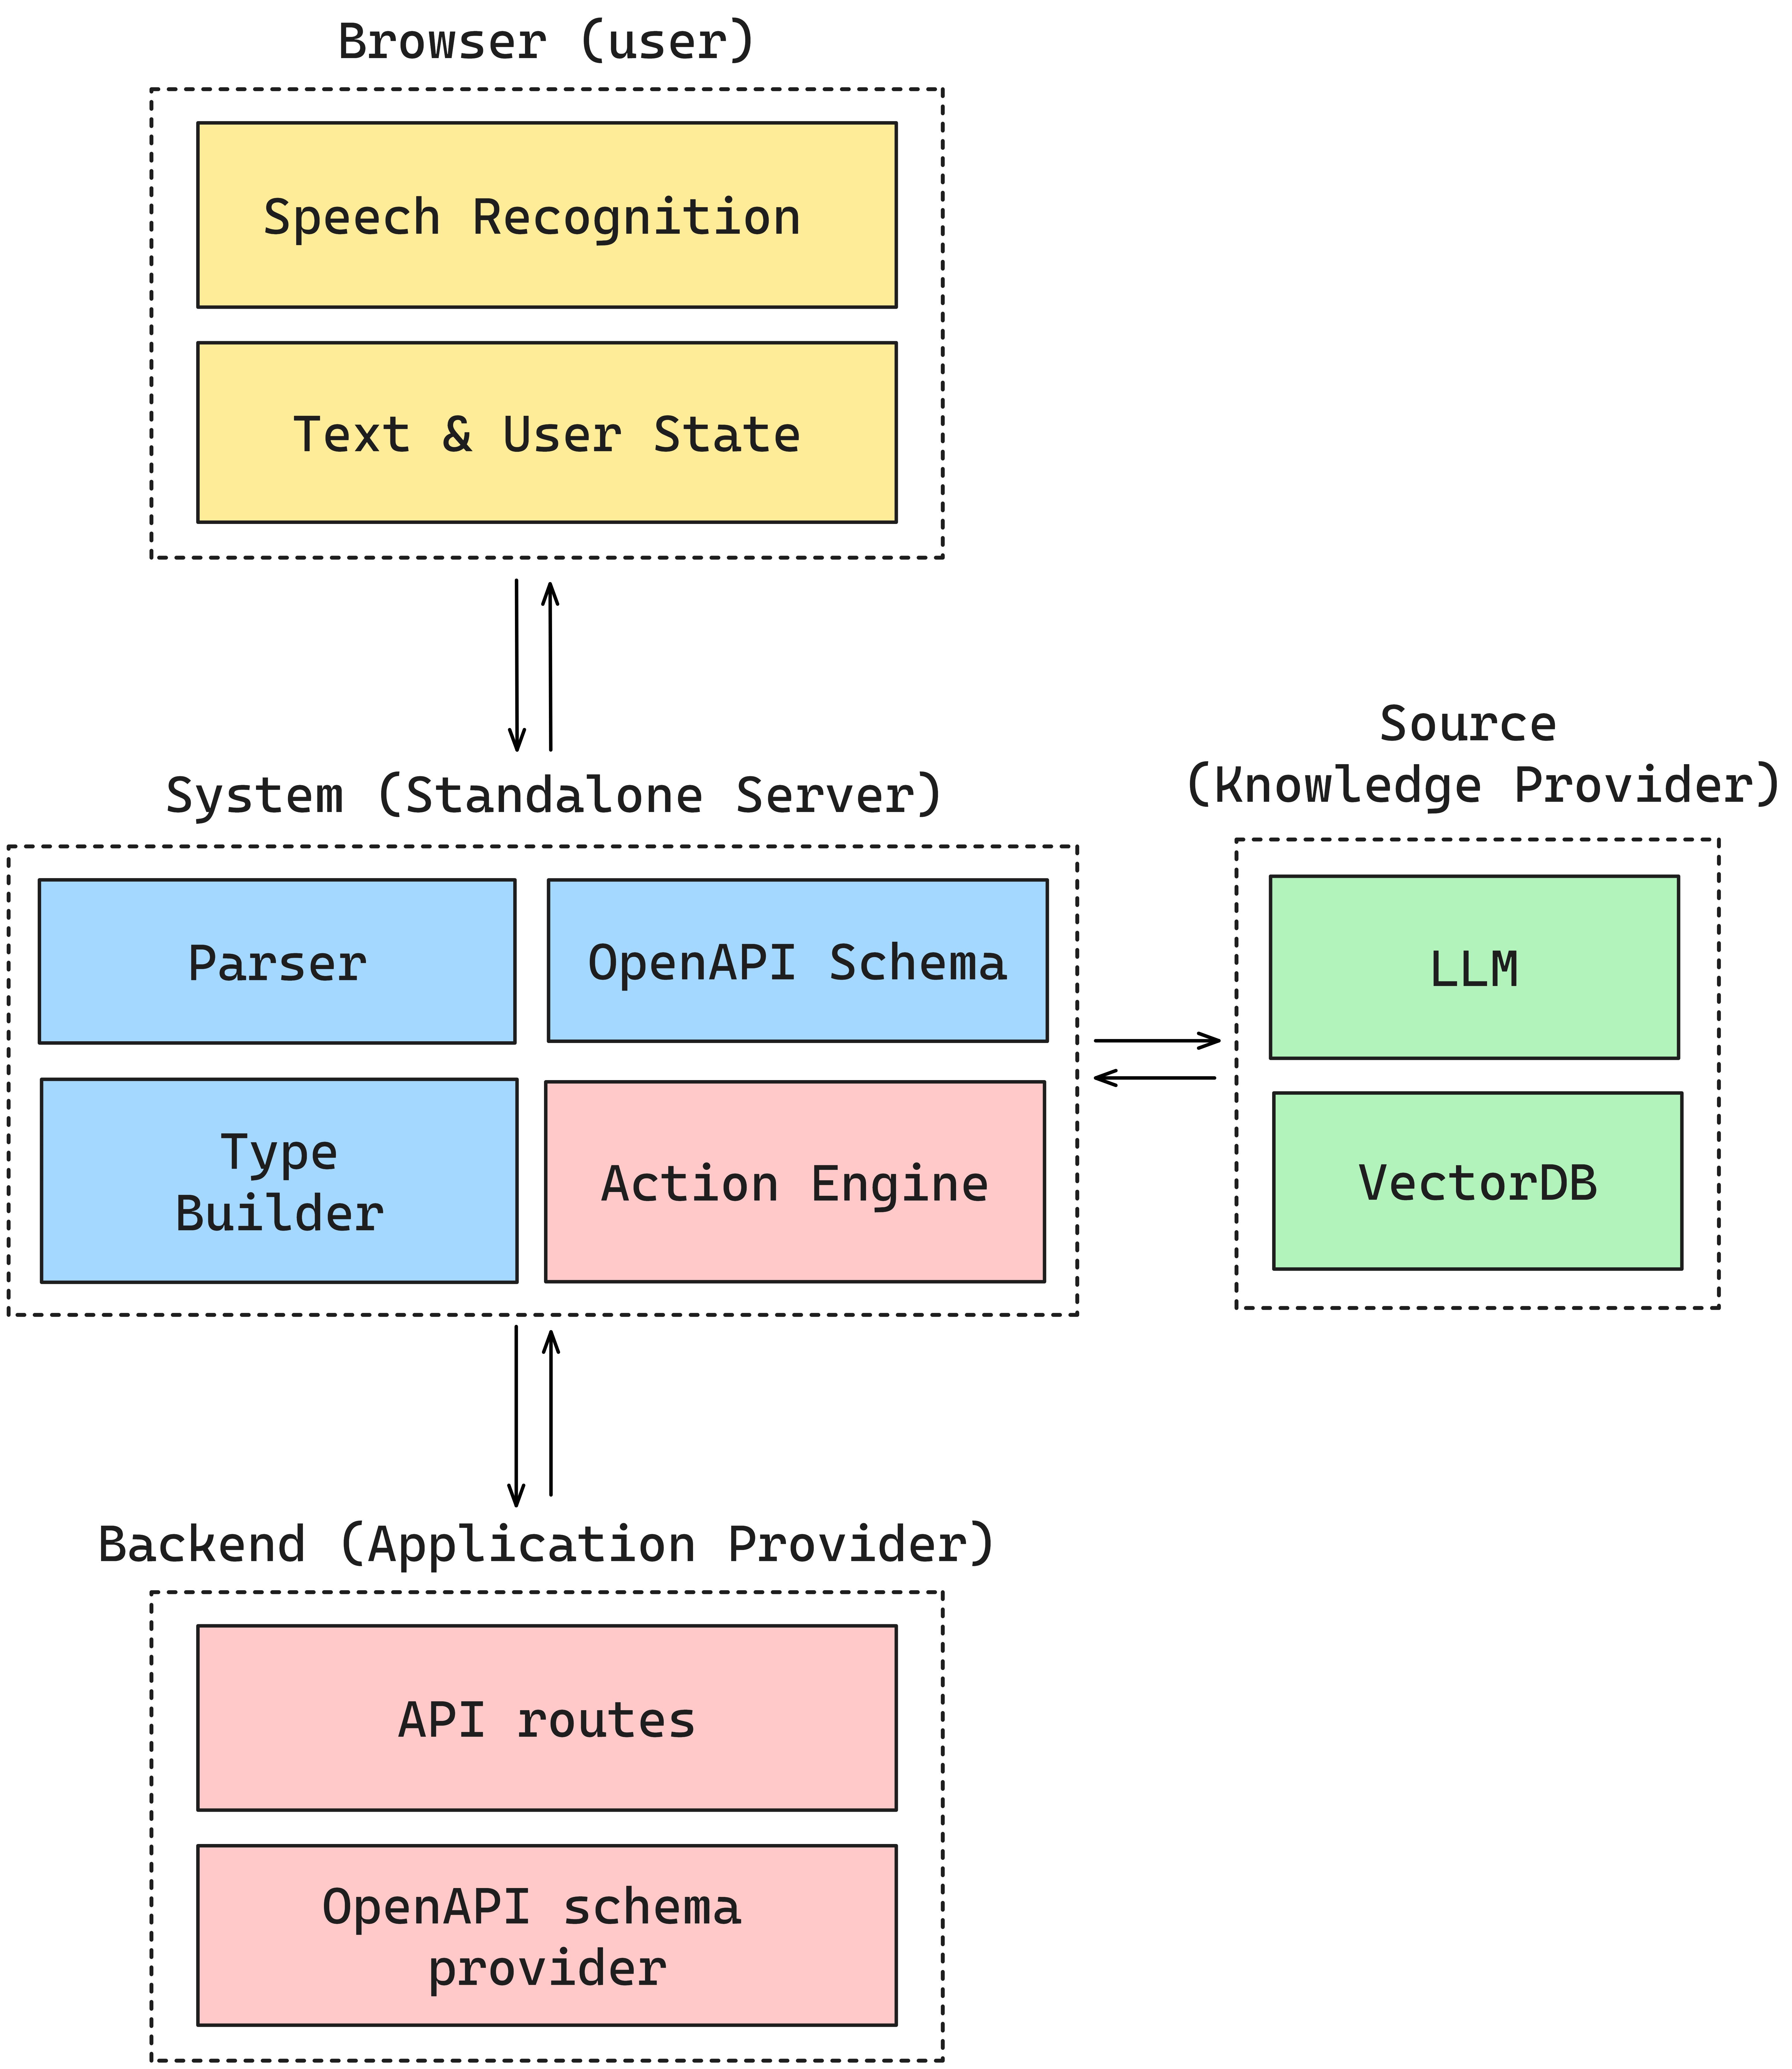
\includegraphics[width=0.48\textwidth]{images/server.png}
    \caption{Server Architecture with Action Model}
    \label{fig}
\end{figure}


\subsection{Action Engine Architecture}
The Action engine architecture follows the same pattern as the build time CLI (CLI that converts the OpenAPI schema to type definitions). An action engine is not an AI system. Currently, it is a simple JSON parser that can understand the JSON data from LLM. It turns the normal Large Language Model into a Simple Action Model, that enables function calling and chaining. 

Let's consider a simple application for mathematical calculations, the user asked ” What is 10 + 2 / 4” and the Action engine had access to all types of mathematical functions. So the LLM returns instructions in JSON tag and the Action engine will execute the function in the order of the instructions. The result is then sent back to the user.


\begin{figure}[htbp]
    \centering
    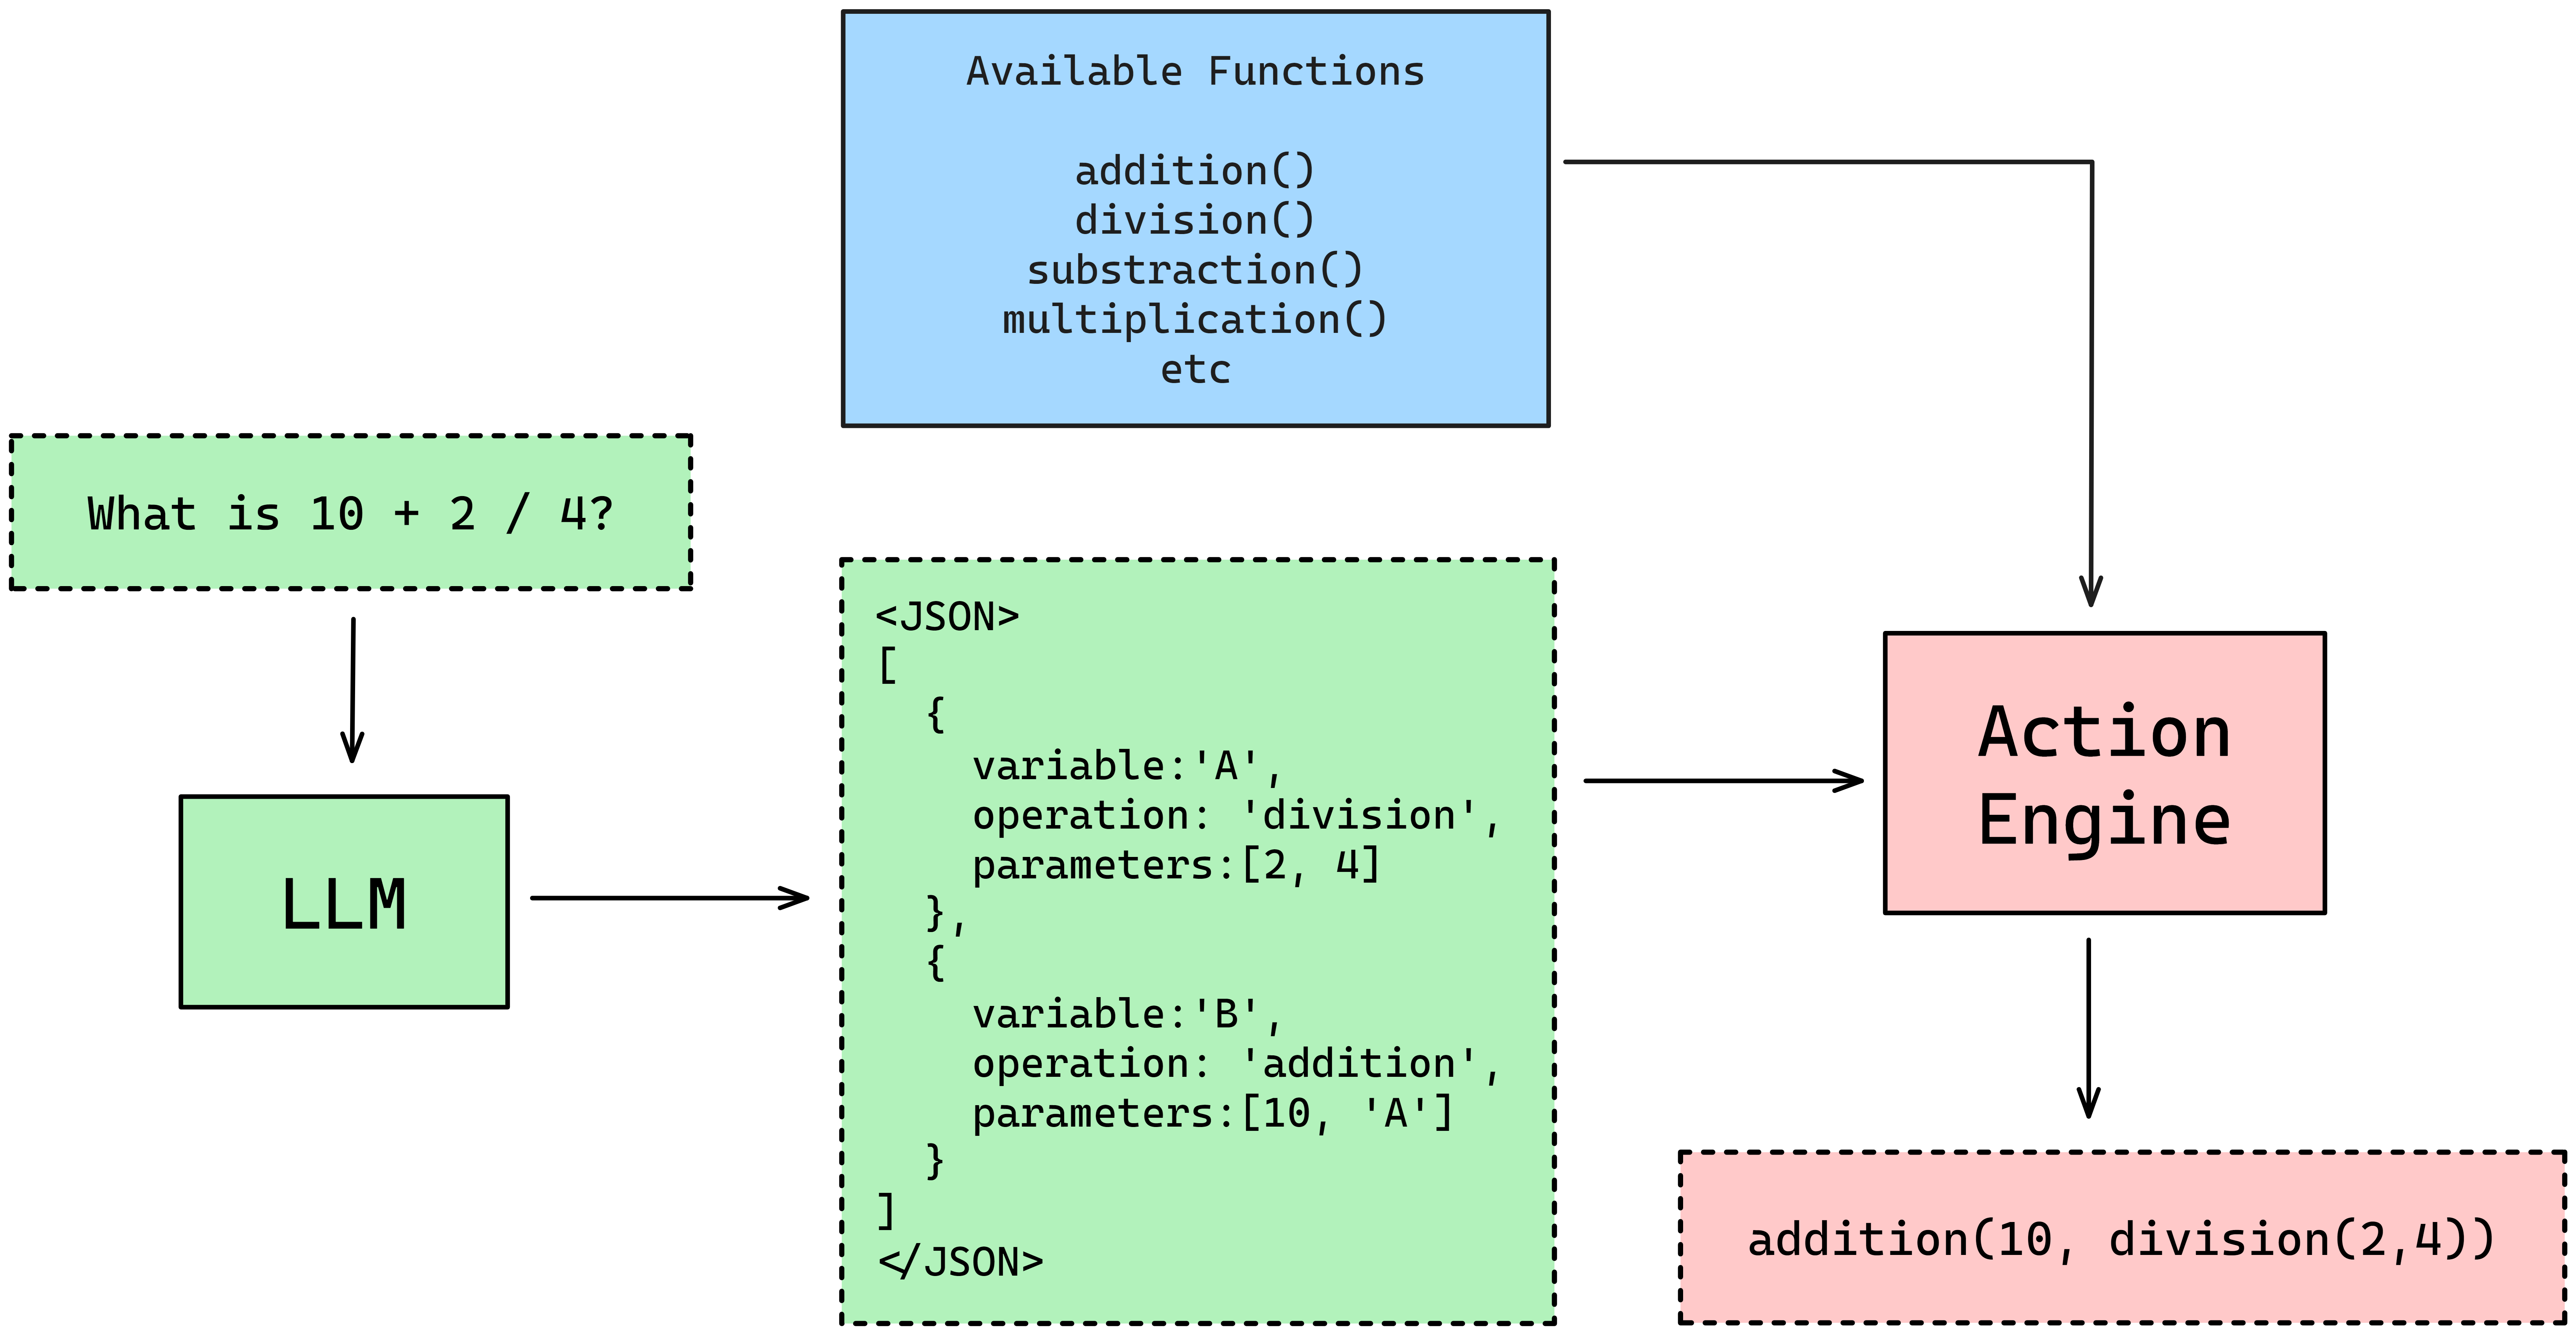
\includegraphics[width=0.48\textwidth]{images/maths.png}
    \caption{Simplified Maths problem done with Function Calling.}
    \label{fig}
\end{figure}

The new unknown variable is generated and used at runtime. The type structure of return JSON can be customized. Here this JSON is enough to represent the environment. JSON is parsed and validated by the engine and array to moved to the execution stack and each function is called sequentially, where the result of the previous execution is stored in the heap at runtime.

\begin{figure}[htbp]
\centering
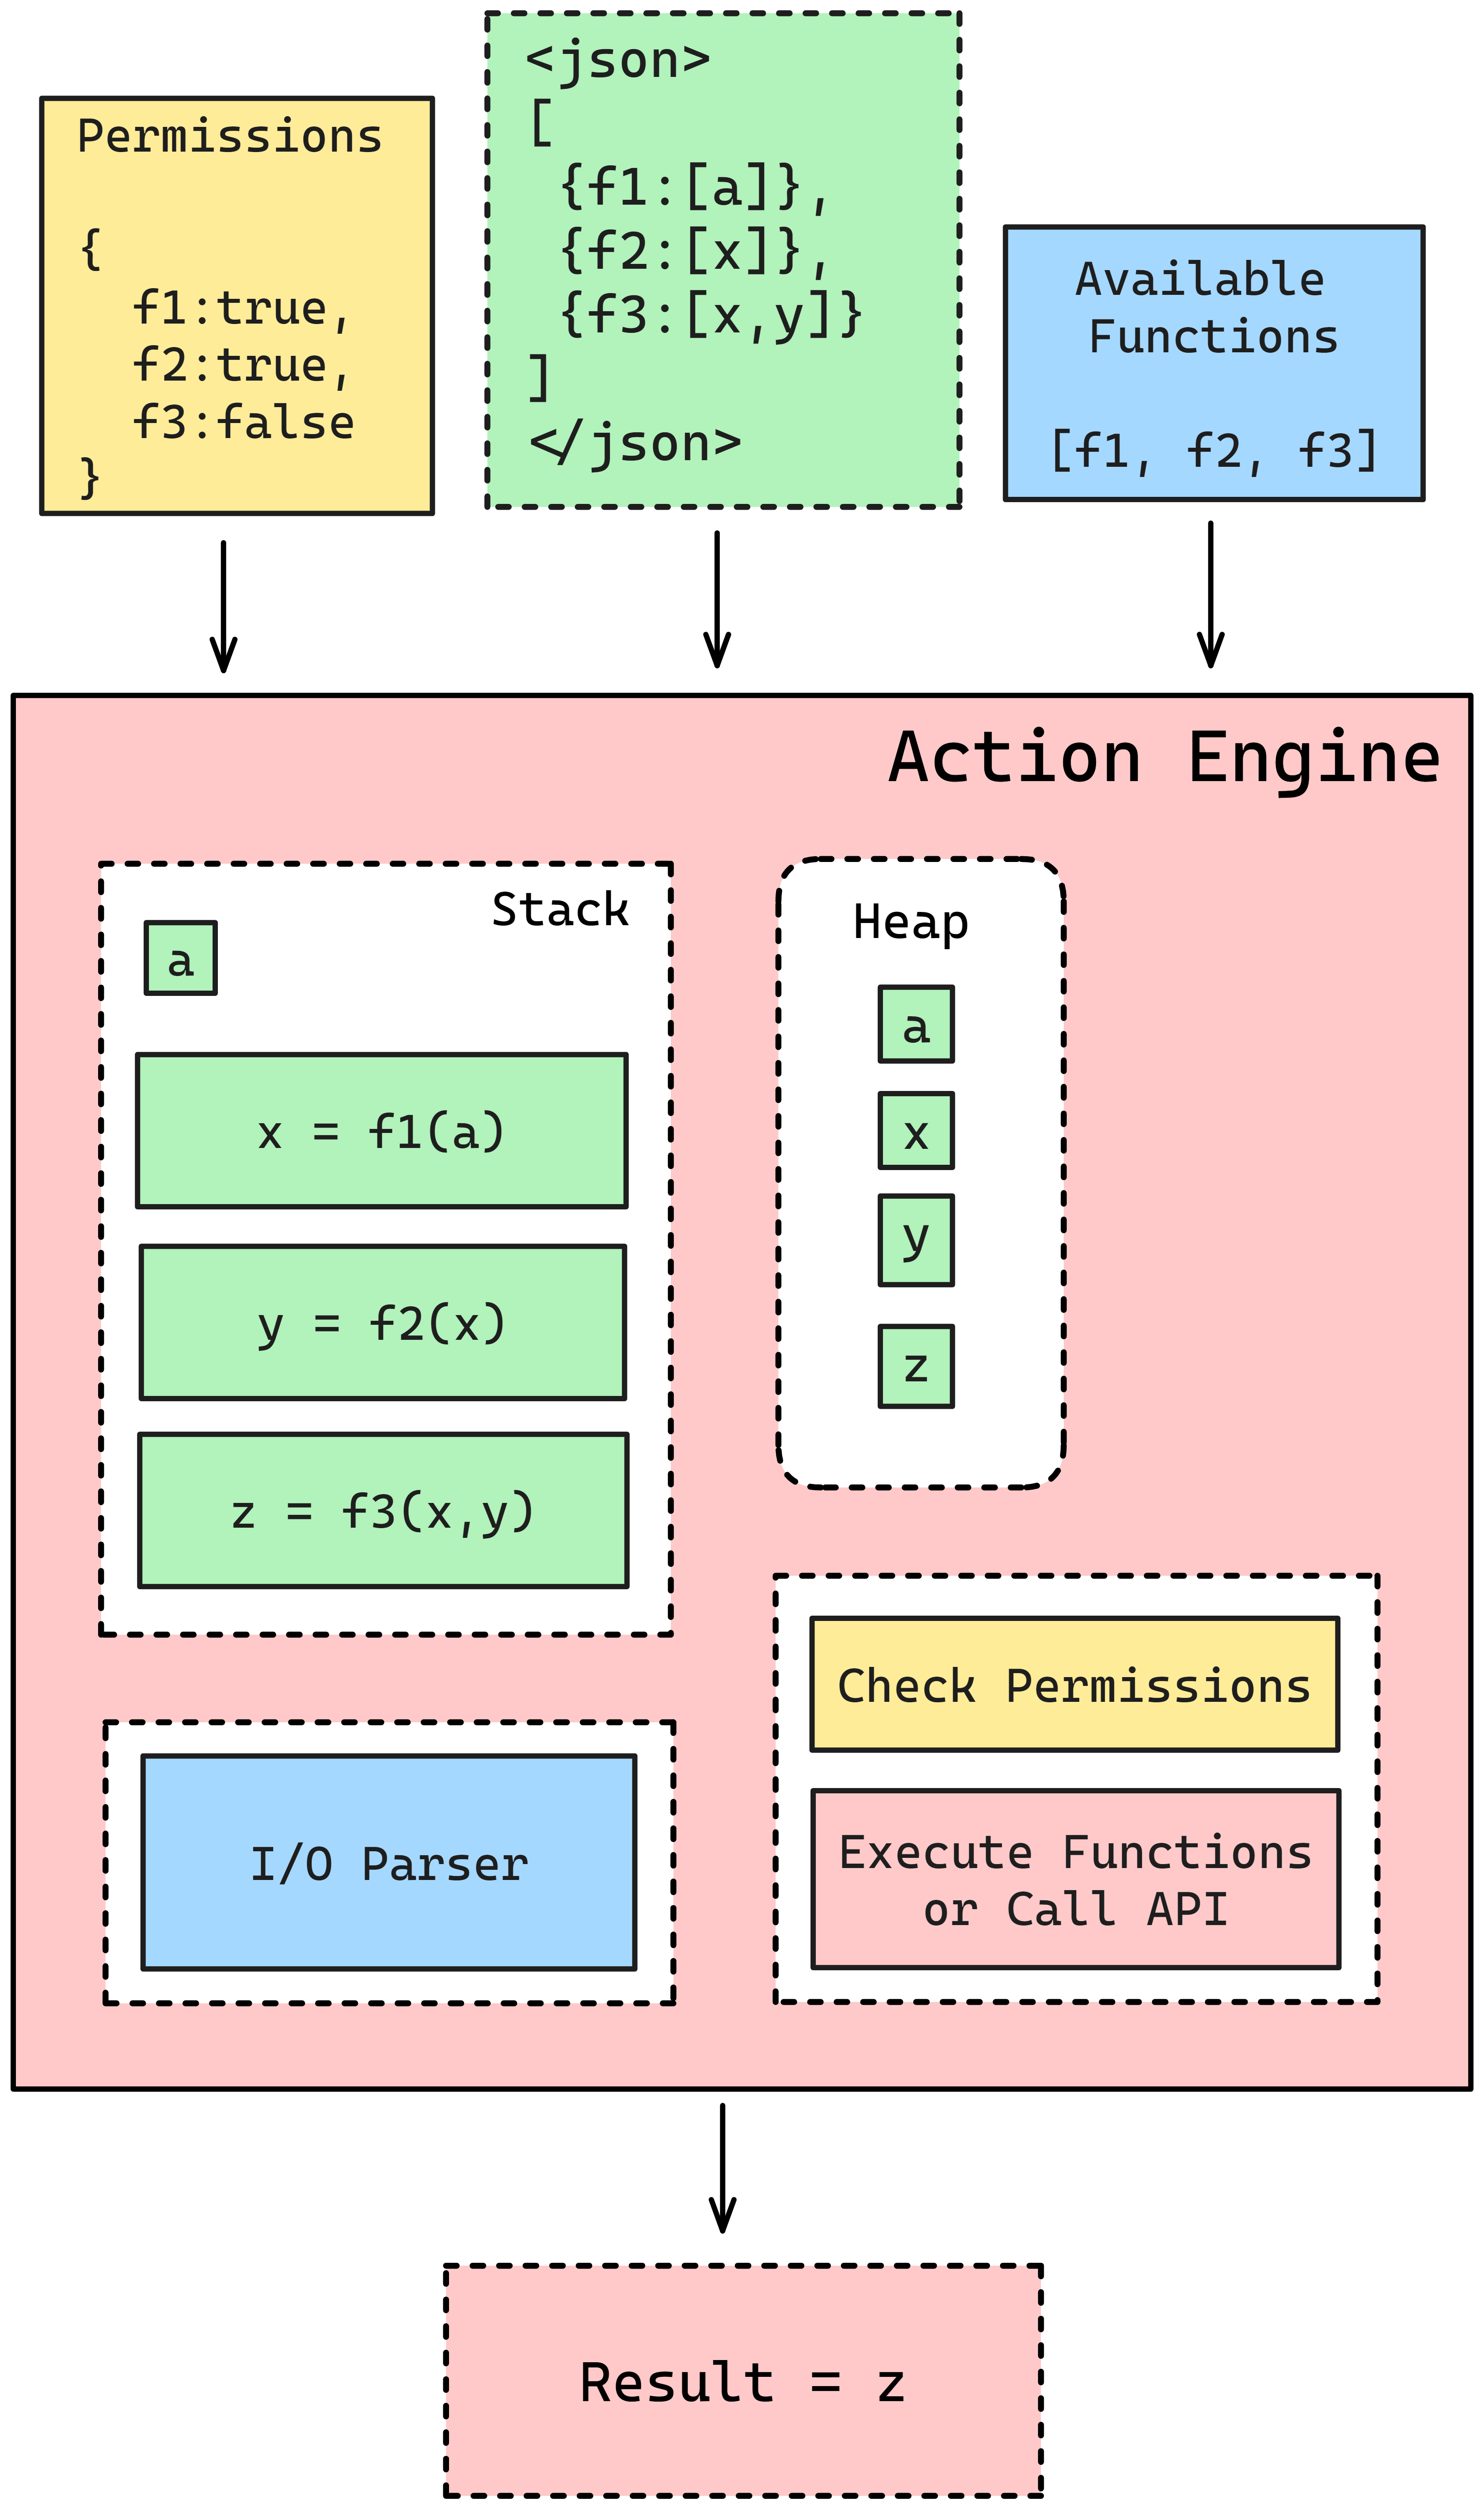
\includegraphics[width=0.48\textwidth]{images/action-engine.png}
\caption{Block Diagram of Action Engine Architecture}
\label{fig}
\end{figure}

Two types of instructions can be evaluated. Single: parse the JSON, execute the function, done. But for multiple sequential instructions require careful validations and parsing. The first execution of the function requires a complete set of parameters. Always store the executed data and function parameters in the heap. If other instructions require data from a previous execution, search in the input params list in a stack or search heap. If data is not found, return an error (and let the server handle that part). 

To ensure consistency and compatibility, the input data parameters and output results from each execution are also validated before passing down to the next instructions. This standardization allows for seamless processing and execution of function calling, enabling the system to effectively detect any instances of an error made by the language model.

The permission is the list of functions that are allowed to run without users' concerns. If a function is true, then execute it without asking for permission. If not then return the current result stack of execution to the user and wait until the user permits. This feature is crucial while building highly secure and user data-dependent applications. Users don’t want any LLM to make decisions and execute some functionalities on its own without their permission.

% \begin{table}[htbp]
% \caption{VGG16 Classifier}
% \label{tab2} % Label for referencing later
% \begin{center}
% \begin{tabular}{|c|c|}
% \hline
% \textbf{VGG16 parameters} & \textbf{parameter values} \\ % Bold headers
% \hline
% Batch size & 32 \\ % Second row
% \hline
% Epochs& 50 \\
% \hline
% Optimizer& adam\\
% \hline
% Class mode& Categorical\\
% \hline
% loss & categorical\_crossentropy \\

% \hline
% %\multicolumn{2}{l}{$^{\text{a}}$Footnote text here.} % Footnote
% \end{tabular}
% \end{center}
% \end{table}





\subsection{Utilizing Vector storage}
Retrieval Augmented Generation (RAG) is a popular technique used alongside with large language models (LLMs) to improve its performance by including external knowledge sources. Mostly here we can utilize it with help of vector databases. 

OpenAPI schema format supports descriptions and examples. These descriptions can be stored in vector database alongside the meta data of each API routes or components. If the application OpenAPI schema is larger than context window capacity of the LLM, then utilization of vector databases can still reduce the no of request to LLMs. Query the vector database with user prompt and get most probable API route or component. Then combine the results with user prompt to get response from LLM. This approach is faster and efficient than querying the LLMs with large amount of OpenAPI schema.

RAG based Action model is much more efficient when it comes to usage of token while querying. Less the no of tokens used, faster the model respond.

\begin{figure}[htbp]
\centering
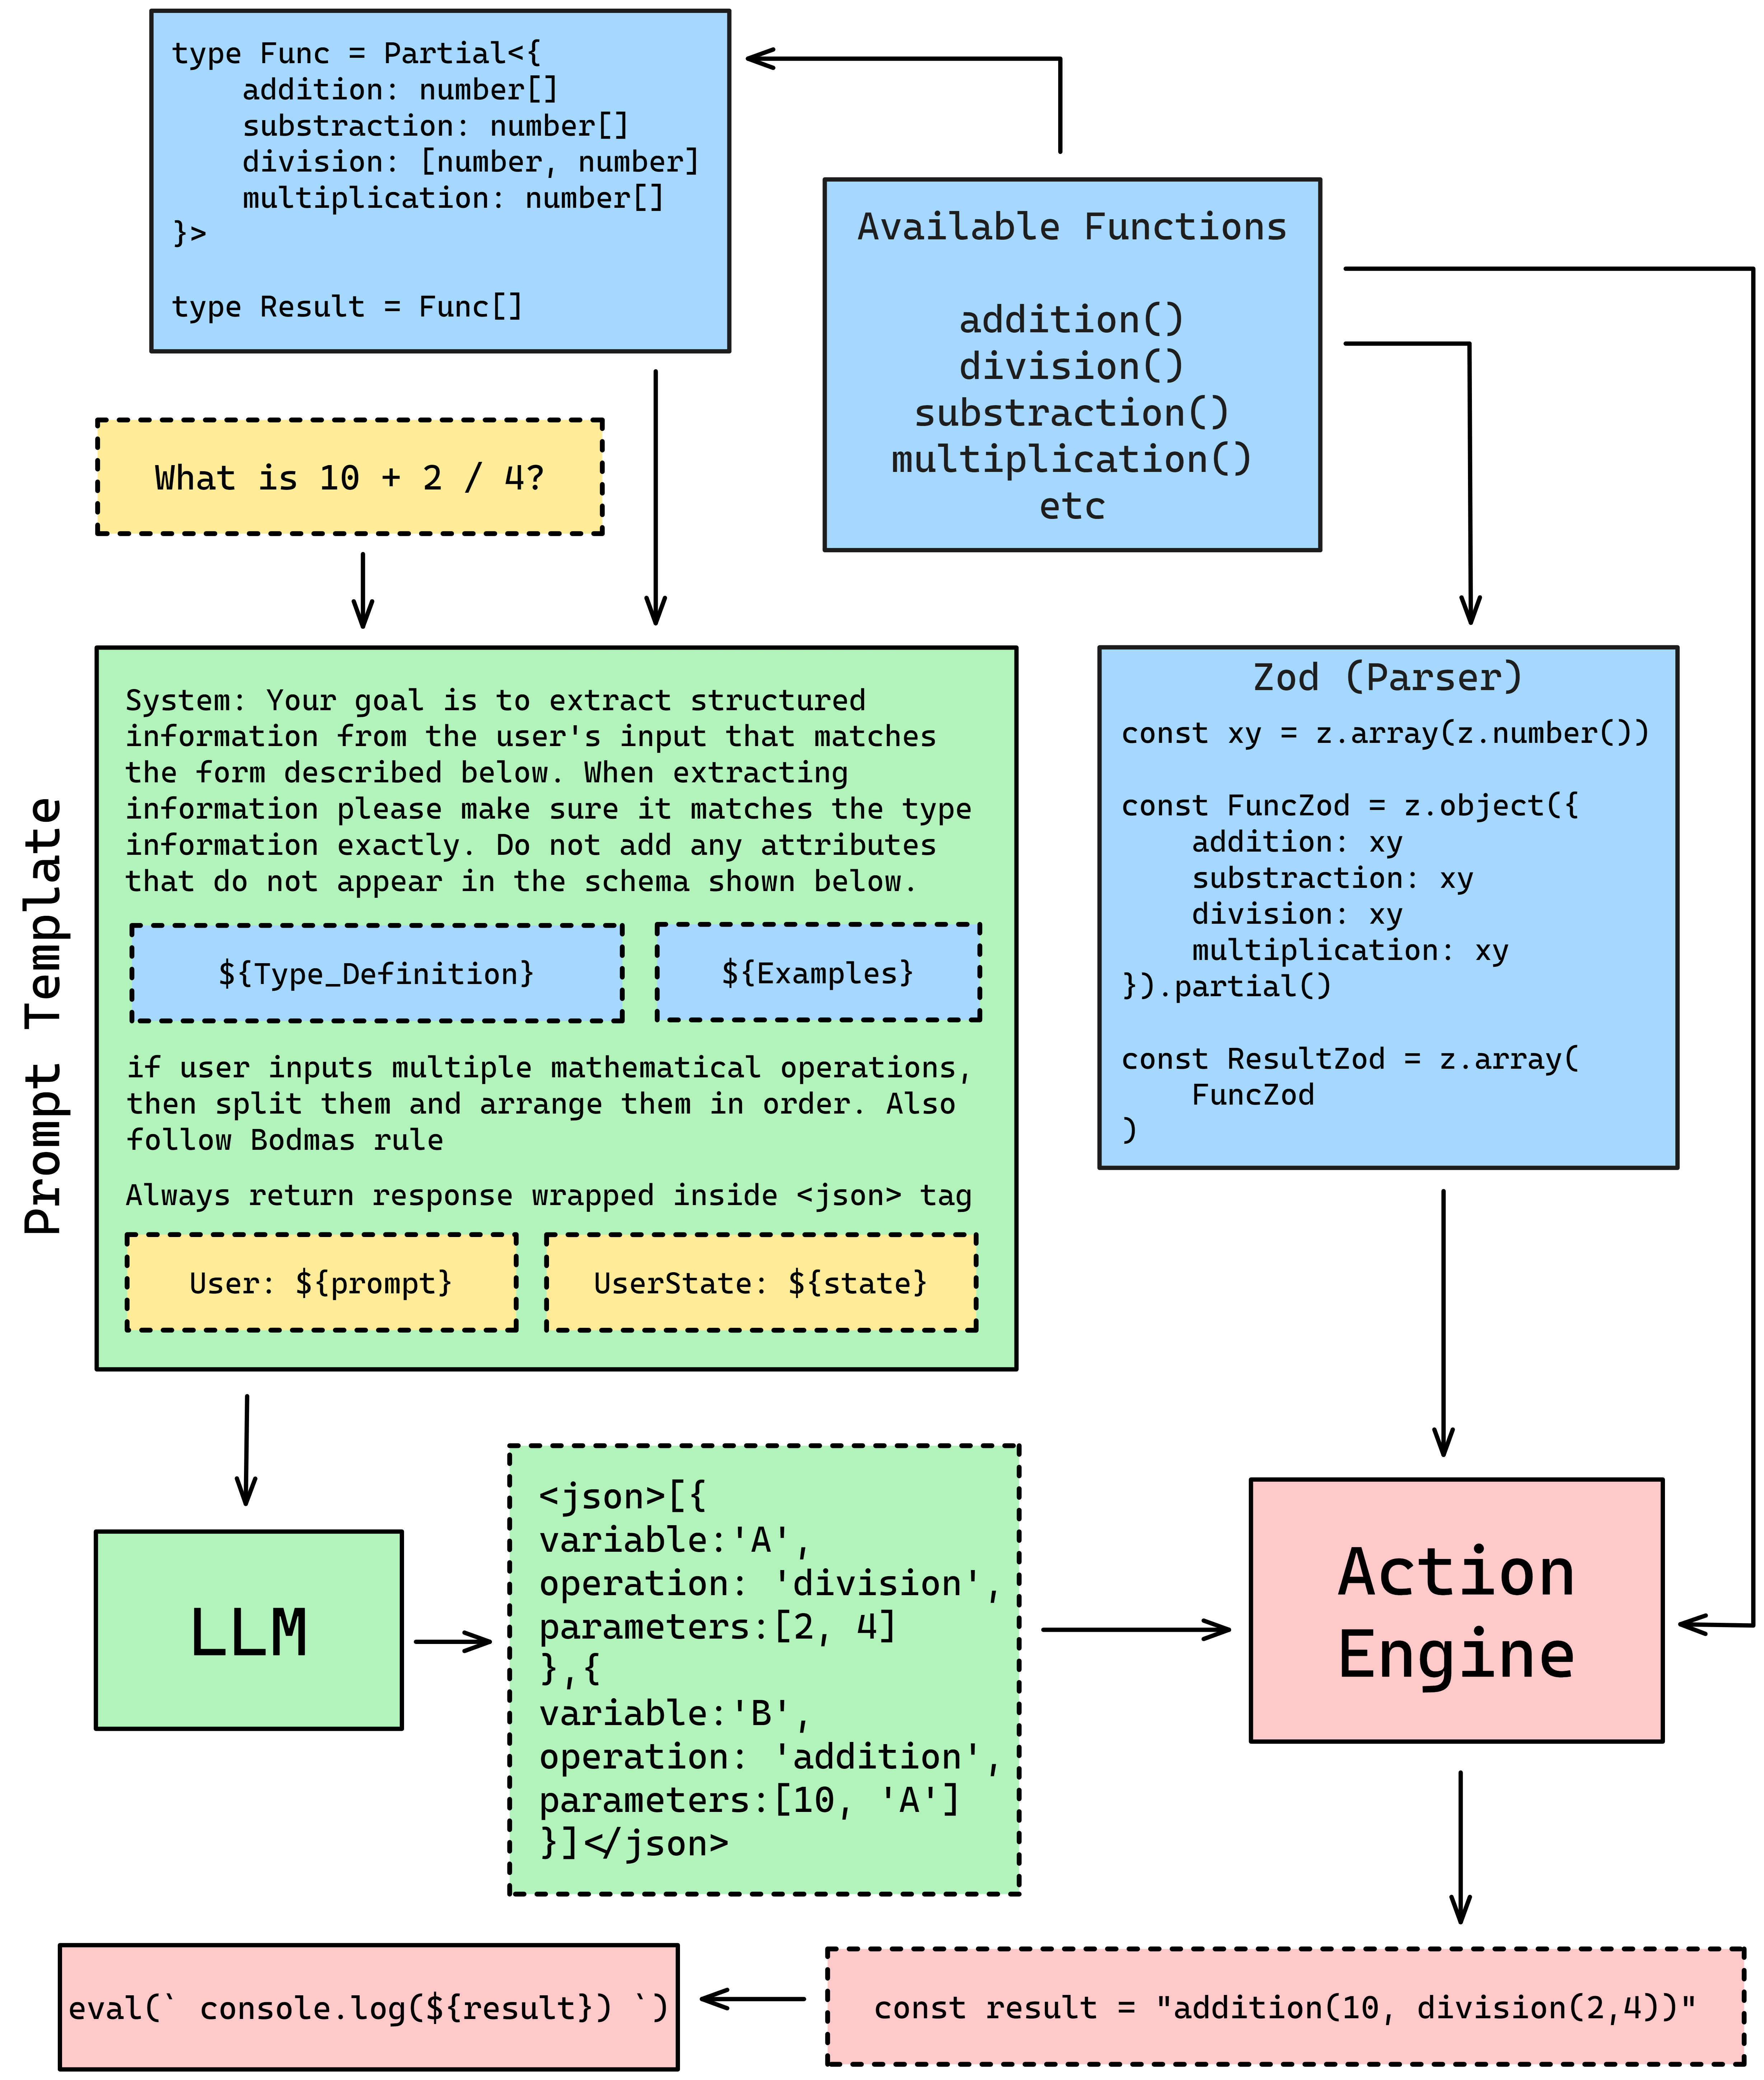
\includegraphics[width=0.48\textwidth]{images/program.png}  
\caption{Detailed Block Diagram of Maths problem}
\label{fig}
\end{figure}


\subsection{Utilizing runtime validations}
Action models requires strict parsing and validations with OpenAPI schema. LLMs hallucinate sometimes, making it untrust worthy to take decisions. That's why it is important to validate the input and output data from fetching the API. But what if the LLM can just go around the world wide web and fetch the schema of the API and validate at runtime and cache it. This approach is much more futuristic than it sounds. The user prompts, LLM looks for relevant schema from Google search and call those APIs. While system is looking for docs, it can build validators and parsers for the schema at runtime. Also utilize caching mechanism to store the build files for future use. 

It's like google search, but instead of querying, it'll do tasks online by itself. An inevitable future of language models. 

\subsection{Utilizing multiple calls to LLM}
Popular function calling projects like ReAct utilizes multiple call to LLM to make sure to get the best result and response is moving in right directions. This approach is also useful in Action model. If the response from LLM is not clear or not understandable, then a second call to LLM can be reduce the errors.

This paper was focused on "how to sequentially function call with one query to LLM". But multiple calls to LLM can be useful in some cases. If return data of previously executed function may not be clear or not understandable. Or the data can so long that, without intermediate assistance, it may not reach the end goal as user expected.

\subsection{Utilizing Program-aided Language Models}
Program-aided Language Models (PALM) are the new architecture of LLMs that are trained on both interpreted programming language and natural languages. These models are utilized with ability to run code directly in system at runtime. This approach is not preferred due to security vulnerabilities like code injection attacks. The `eval()` function allows executing arbitrary code passed as a string. So LLM might execute malicious codes.

Extra runtime linting feature can avoid this vulnerabilities. 
PAL give LLM model extra access to run the code directly into the environment. This approach is suitable for building OpenAPI to function calling tool chain system.

\section{Implementation and Result}
\subsection{Implementation}
From a developer perspective, the implementation of the Sequential Function Calling Tool Chain System involves the following steps:

- Preparation of the OpenAPI schema: The developer fetches the OpenAPI schema from the backend application and prepares the schema at build time. The schema is then converted to type definitions and saved in a folder.

- Preparation of the prompt template: The developer prepares the prompt for the LLM, ensuring that the LLM response is in the correct format. Prompt template includes the necessary type definitions, instructions, and examples as few-shot learning.

- Server architecture: The developer must turn this into a standalone backend server that listens to end users prompts. The server takes the user prompt, combine it into template and sends to LLM. The LLM response is then parsed and sent to the Action engine. Action engine in the next step requires a fetching client library like axios (npm) or tRPC (npm). The result is then sent back to the user in JSON format or streamed as Generative UI (use Next.js or Nuxt.js for server side rending components).

- Action engine architecture: The Action engine is a JSON parser that understands the JSON data from the LLM, use kor (pip) or ai-SDK (npm). It turns the LLM into a Simple Action Model that enables function calling and chaining. The engine executes the functions in the order of the instructions and sends the result back to the user. For implementing the engine, use AI-SDK from Vercel (npm) or popular AI library LangChain (npm, pip) as base ai agent.


\subsection{Performance Evaluation}
Popular LLM benchmarks tools have 4 common metrics to consider in turning into Action Models. They are MMLU (Massive Multitask Language Understanding), Context window size and Median (inference speed or token/second). 

Better the MMLU, better the model can understand the environment. More context window, gives more access to openAPI schema. Faster the inference speed, faster the model can respond with JSON. Context window and Median are inversely proportional. 

If architecture is extended to Program-aided Language Models (PAL), then fine tuning the model with corresponding programming language and documentation of fetching libraries using can improve quality of the responses.



% \begin{figure}[htbp]
% \centering
% 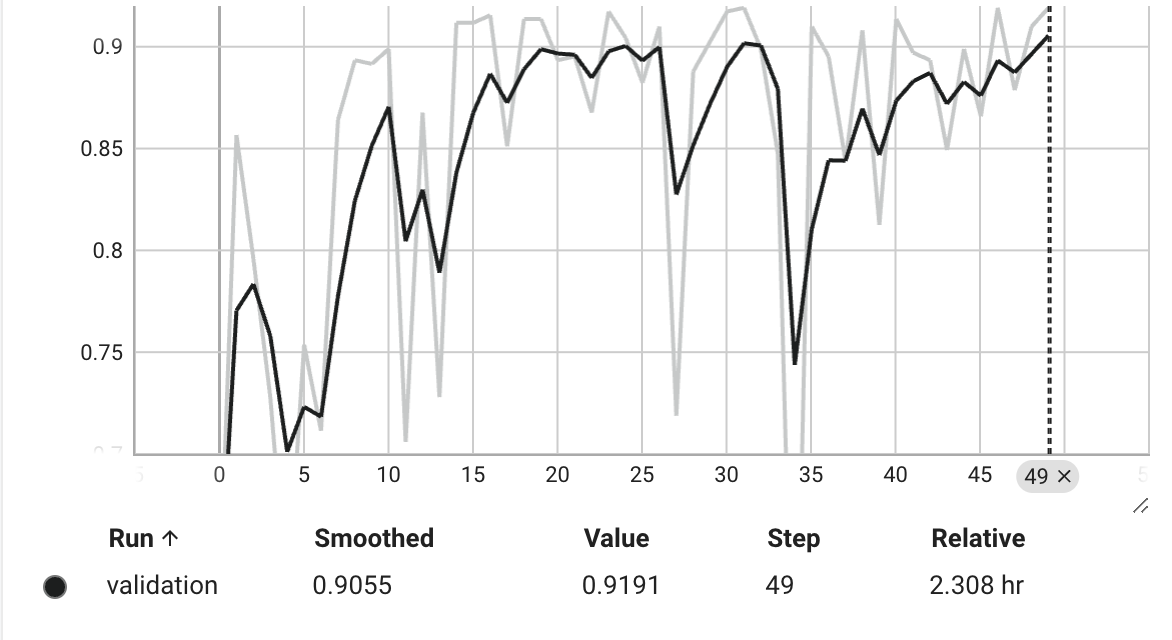
\includegraphics[width=0.48\textwidth, height=7cm]{images/Vgg16acc.png}  
% \caption{Accuracy of Vgg16}
% \label{fig}
% \end{figure}



% \begin{table}[htbp]
% \caption{Performance Evaluation:YOLOv8}
% \label{tab2} % Label for referencing later
% \begin{center}
% \begin{tabular}{|c|c|}
% \hline
% \textbf{Metric} & \textbf{YOLOv8} \\ % Bold headers
% \hline
% Accuracy & 95\% \\ % Second row

% \hline
% Precision&0.94\\
% \hline
% Recall&0.96\\
% \hline
%  F1-score&0.95 \\

% \hline
% %\multicolumn{2}{l}{$^{\text{a}}$Footnote text here.} % Footnote
% \end{tabular}
% \end{center}
% \end{table}


\begin{table}[htbp]
    \centering
    \caption{Performance metrics comparison for Large Language Models}
    \begin{tabular}{|c|c|c|c|c|}
      \hline
      Model & 
      INDEX & 
      \begin{tabular}[c]{@{}l@{}}Context\\    \\ Window\end{tabular} & MMLU & 
      \begin{tabular}[c]{@{}l@{}}MEDIAN\\    \\ (Tokens/s)\end{tabular} \\
      \hline
      claude-3-opus & 100 & 200k & 0.868 & 27.5 \\
      \hline
      gpt-4 & 90 & 8k & 0.864 & 17.5 \\
      \hline
      Llama3-70b & 88 & 8k & 0.82 & 307.3 \\
      \hline
      claude-3-sonnet & 85 & 200k & 0.79 & 59.4 \\
      \hline
       Mixtral-8x22B & 83 & 65k & 0.77752 & 49.9 \\
      \hline
      claude-3-haiku & 78 & 200k & 0.752 & 85.4 \\
      \hline
      claude-instant & 65 & 100k & 0.734 & 84.2 \\
      \hline
      mixtral-8x7b & 68 & 16k & 0.706 & 117.1 \\
      \hline
      gpt-3.5-turbo & 67 & 16k & 0.7 & 58.5 \\
      \hline
      gpt-35-turbo & 67 & 16k & 0.7 & 54 \\
      \hline
      llama2-70b-4096 & 56 & 4k & 0.689 & 251.5 \\
      \hline
      llama-3-8b & 58 & 8k & 0.684 & 121.4 \\
      \hline
      Llama3-8b-8192 & 58 & 8k & 0.684 & 920.8 \\
      \hline
      mistral-7b & 40 & 16k & 0.625 & 102.9 \\
      \hline
      llama-2-13b & 37 & 4k & 0.536 & 115.3 \\
      \hline
      llama-2-7b & 27 & 4k & 0.458 & 204.7 \\
      \hline
      \multicolumn{5}{l}{ArtificialAnalysis/LLM-Performance-Leaderboard.}
    \end{tabular}
  \end{table}

The evaluation of these models are provided by ArtificialAnalysis/LLM-Performance-Leaderboard from hugging face. The evaluation is based on the following metrics: API ID, INDEX (Normalized avg), CONTEXT WINDOW, MMLU, MEDIAN (Tokens/s). The evaluation is based on the performance of the models in terms of their ability to generate human-like text, understand and respond to user queries, and provide accurate and relevant information. The models are ranked based on their performance across these metrics, with higher scores indicating better performance

However, it is essential to note that increasing the parameter count does not always guarantee better performance. The model's architecture, training data, and fine-tuning processes also play crucial roles in determining its overall capabilities. Therefore, it is essential to consider these factors in conjunction with the parameter count to assess the model's performance accurately. From a perspective of Enterprise, the model has to be open source or they can't fine tune the model with their own custom dataset. Fine tuning on their specialized environment can help to gain more context window through each instance of request.

\subsection{Findings}
From Fig. 6, which illustrates the usefulness of the Program-aided Language Models (PALM) combined with the OpenAPI Action Engine. Also introducing external vector knowledge base into this architecture brings more efficiency and speed to the system.
The following are the main findings:
\begin{enumerate}
    \item  High speed response: Vector knowledge base of OpenAPI type definition reduce time to searching and faster response from system
    \item Less usage of token: Splitting the OpenAPI type definition into chunks and vector embedding, brings faster response with lesser prompting token size.
     \item Less complexity: The system is less complicated compared to Chain-of-Thought Prompting (COT) or Tree of Thoughts (TOT) architecture. This system is much more simpler and efficient, because of single query to LLM.
     \item Reduction on computation: The system is much more efficient in terms of computation. The system is much more faster and efficient than other systems.
    \item Practical Deployment: We have developed a practical and
    easily understandable applications build on top of this system. An banking app that navigates through the API routes and help user navigates applications with prompts.
\end{enumerate}


By providing a user-friendly interface for users, this system makes real-time navigates and assistance possible. The system is also capable of handling complex requirements and executing multiple functions sequentially, making it a valuable tool for developers and users alike.

\subsection{Comparison with State-of-the-Art Models}
The system was compared with other state-of-the-art models, such as ReAct and Chain-of-Thought Prompting (COT). The system outperformed these models in terms of speed, efficiency, and accuracy. The system was also found to be more user-friendly and easier to use than other models. The system's ability to execute multiple functions sequentially with a single query to the LLM makes it a valuable tool as wrapper around consumer applications.

Most popular LLM inference provider now supports function calling. ChatGPT from OpenAI, Sonnet from Claude.ai, and many more. But these models are not good enough to execute multiple functions sequentially. 

Recently CDN provider Cloudflare released OpenAPI schema to function calling toolkit (@cloudflare/ai-utils). But they use runtime parser building and validations. This paper is a step behind of that. They use more tokens in-context learning to represent type definition, because they use standard Object definition in JSON format. But this paper is more focused on type definition in typescript language object JSON and parsing through zod (npm) library.

% \begin{table}[htbp]
% \caption{Comparison of the Performance Metrics for VGG16 and AlexNet}
% \label{tab2} % Label for referencing later
% \begin{center}
% \begin{tabular}{|c|c|c|}
% \hline
% \textbf{Metric} & \textbf{VGG16} & \textbf{AlexNet} \\ % Bold headers
% \hline
% Accuracy & 92\% & 64\%\\ % Second row

% \hline
% Loss&68&76\\
% \hline

% %\multicolumn{2}{l}{$^{\text{a}}$Footnote text here.} % Footnote
% \end{tabular}
% \end{center}
% \end{table}



% \begin{figure}[htbp]
% \centering
% 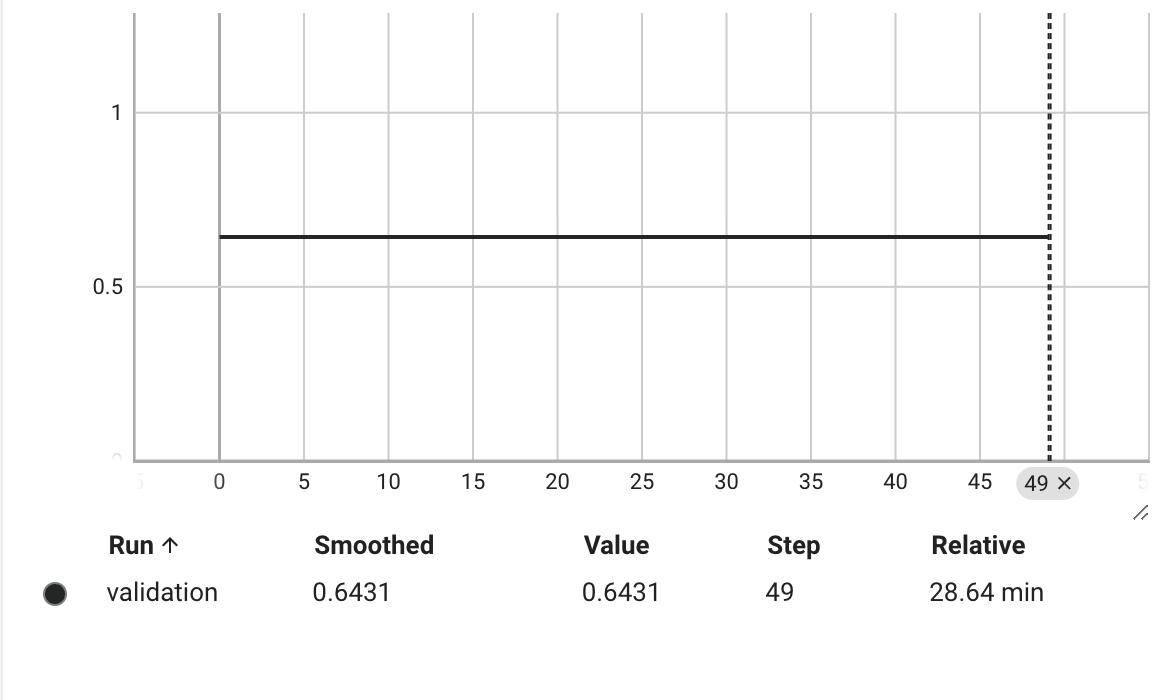
\includegraphics[width=0.48\textwidth, height=7cm]{images/AlexNet.png}  
% \caption{Accuracy of AlexNet}
% \label{fig}
% \end{figure}



\section{Conclusion}
Everyday new sophisticated models are launching and breaking the records. The competition for building the best language model has two categories. One, model that knows everything about the world and can answer any questions. Two, model that run on any small devices. Consumer who can afford large and faster cloud inference provider don't really care about privacy or external knowledge base. But the open source community focused on building personal model that run on any small devices. That's where projects like this paper comes in. Enabling the LLM to research through the internet and execute actions makes the devices more smarter and efficient. Also ensuring the privacy and security of the user data.

Depending ont the use case, models, computation cost, and size of schema, the system can be customized to meet the specific requirements of the application. The system can be easily integrated into existing applications for better user experiences. 

We are actively pursuing these lines of inquiry, with the goal of translating our theoretical framework into practical, real-world applications. Our findings are useful, but it's important to note that this is just the beginning of a bigger research project. AI systems are complex, and there's still a lot to learn and improve in our approach. To sum up, this paper is an important step in our research, but it's also a starting point for more work to come. We're excited to share updates as we continue our work and try to bridge the gap between research ideas and practical AI applications in the real world.


\begin{thebibliography}{00}
    \bibitem{bib0}
    Luyu Gao, Aman Madaan, Shuyan Zhou, Uri Alon, Pengfei Liu, Yiming Yang, Jamie Callan, Graham Neubig~(Jan 2023), 
    {\it PAL: Program-aided Language Models}, 
    arXiv/Computer Science/Computation and Language,
     arXiv:2211.10435v2.
    
    \bibitem{bib1}
    Tatsuro Inaba, Hirokazu Kiyomaru, Fei Cheng, Sadao Kurohashi~(2023)
    {\it MultiTool-CoT: GPT-3 Can Use Multiple External Tools with Chain of
    Thought Prompting}, arXiv/Computer Science/Computation and Language,
     arXiv:2305.16896v1
    
    \bibitem{bib2}
    Yujia Qin, Shihao Liang, Yining Ye, Kunlun Zhu, Lan Yan, Yaxi Lu, Yankai Lin, Xin Cong, Xiangru Tang, Bill Qian, Sihan Zhao, Lauren Hong, Runchu Tian, Ruobing Xie, Jie Zhou, Mark Gerstein, Dahai Li, Zhiyuan Liu, Maosong Sun~(2023)
    {\it TOOLLLM: FACILITATING LARGE LANGUAGE
    MODELS TO MASTER 16000+ REAL-WORLD APIS}, arXiv/Computer Science/Artificial Intelligence,
    arXiv:2307.16789v2 
    .
    
    \bibitem{bib3}
    Sehoon Kim, Suhong Moon, Ryan Tabrizi, Nicholas Lee, Michael W. Mahoney, Kurt Keutzer, Amir Gholami~(Jun 2024) 
    {\it An LLM Compiler for Parallel Function Calling},
    arXiv/Computer Science/Computation and Language,
    arXiv:2312.04511v3.
    
    \bibitem{bib4}
    Jason Wei, Xuezhi Wang, Dale Schuurmans, Maarten Bosma, Brian Ichter, Fei Xia, Ed Chi, Quoc Le, Denny Zhou~(Jan 2023 )
    {\it Chain-of-Thought Prompting Elicits Reasoning
    in Large Language Models}, arXiv/Computer Science/Computation and Language,
    arXiv:2201.11903v6 .
    
    \bibitem{bib5}
    Zekun Li, Baolin Peng, Pengcheng He, Michel Galley, Jianfeng Gao, Xifeng Yan~( Feb 2023)
    {\it Guiding Large Language Models via
    Directional Stimulus Prompting} 
    arXiv/Computer Science/Computation and Language,  arXiv:2302.11520v4 .
    
    
    \bibitem{bib6}
    Lei Wang, Chen Ma, Xueyang Feng, Zeyu Zhang, Hao Yang, Jingsen Zhang, Zhiyuan Chen, Jiakai Tang, Xu Chen, Yankai Lin, Wayne Xin Zhao, Zhewei Wei, Ji-Rong Wen~(Apr 2024){\it A Survey on Large Language Model based Autonomous
    Agents},arXiv/Computer Science/Artificial Intelligence, arXiv:2308.11432v5 .
    
    \bibitem{bib7}
    Shunyu Yao, Dian Yu, Jeffrey Zhao, Izhak Shafran, Thomas L. Griffiths, Yuan Cao, Karthik Narasimhan,~(Dec 2023){\it Tree of Thoughts: Deliberate Problem Solving
    with Large Language Models}, arXiv/Computer Science/Computation and Language,  arXiv:2305.10601v2.
    
    \bibitem{bib8}
    Qingxiu Dong, Lei Li, Damai Dai, Ce Zheng, Jingyuan Ma, Rui Li, Heming Xia, Jingjing Xu, Zhiyong Wu, Baobao Chang, Xu Sun, Lei Li, Zhifang Sui.~(Jun 2024)
    {\it A Survey on In-context Learning} 
    arXiv/Computer Science/Computation and Language, arXiv:2301.00234v4.
    
    \bibitem{bib9}
    Shunyu Yao, Jeffrey Zhao, Dian Yu, Nan Du, Izhak Shafran, Karthik Narasimhan, Yuan Cao~( Mar 2023 )
    {\it REACT: SYNERGIZING REASONING AND ACTING IN
    LANGUAGE MODELS},arXiv/Computer Science/Computation and Language, arXiv:2210.03629v3 .

    \bibitem{bib10}
Ruoxi Sun, Sercan Ö. Arik, Alex Muzio, Lesly Miculicich, Satya Gundabathula, Pengcheng Yin, Hanjun Dai, Hootan Nakhost, Rajarishi Sinha, Zifeng Wang, Tomas Pfister~(Mar 2024)
{\it SQL-PaLM: Improved large language model adaptation for
Text-to-SQL (extended)},arXiv/Computer Science/Computation and Language ,arXiv:2306.00739v4.



\bibitem{bib11}
Yujia Qin, Shengding Hu, Yankai Lin, Weize Chen, Ning Ding, Ganqu Cui, Zheni Zeng, Yufei Huang, Chaojun Xiao, Chi Han, Yi Ren Fung, Yusheng Su, Huadong Wang, Cheng Qian, Runchu Tian, Kunlun Zhu, Shihao Liang, Xingyu Shen, Bokai Xu, Zhen Zhang, Yining Ye, Bowen Li, Ziwei Tang, Jing Yi, Yuzhang Zhu, Zhenning Dai, Lan Yan, Xin Cong, Yaxi Lu, Weilin Zhao, Yuxiang Huang, Junxi Yan, Xu Han, Xian Sun, Dahai Li, Jason Phang, Cheng Yang, Tongshuang Wu, Heng Ji, Zhiyuan Liu, Maosong Sun~(Jun 2023)
{\it Tool Learning with Foundation Models},arXiv/Computer Science/Computation and Language,  arXiv:2304.08354v2,Jun 2023.


\bibitem{bib12}
T. B. Brown, B. Mann, N. Ryder, M. Subbiah, J. Kaplan, P. Dhariwal, A. Neelakantan, P. Shyam, G. Sastry, A. Askell, S. Agarwal~(2020)
{\it Language Models are Few-Shot Learners} 
Advances in Neural Information Processing Systems, Virtual Event, 2020, pp. 1871-1882, doi: 10.5555/3326943.3327012.



\bibitem{bib13}
J. Smith, K. Johnson, L. Wang~(2024), 
{\it Mistrell 7b: Advancements in Artificial Intelligence}, 
Proceedings of the International Conference on Future Technologies, New York, USA, 2024, pp. 100-105, doi: 10.1109/CONFERENCE12345.2024.678910.


\bibitem{bib14}
John Doe, Jane Smith, David Johnson~(2023)
{\it LLaMA: Open and Efficient Foundation}
 Proceedings of the International Conference on Computational Intelligence, Communication Technology and Networking (CICTN), Ghaziabad, India, 2023, pp. 563-568, doi:10.1109/CICTN57981.2023.10141447.


\bibitem{bib15}
J. Wu et al.~(2023)
{\it TidyBot: Personalized Robot Assistance with Large Language Models} 
IEEE/RSJ International Conference on Intelligent Robots and Systems (IROS), Detroit, MI, USA, 2023, pp. 3546-3553, doi: 10.1109/IROS55552.2023.10341577.

\end{thebibliography}

% \section*{References}
% [1] Luyu Gao, Aman Madaan, Shuyan Zhou, Uri Alon, Pengfei Liu, Yiming
% Yang, Jamie Callan, Graham Neubig (Jan 2023), PAL: Program-aided
% Language Models, arXiv/Computer Science/Computation and Language,
% arXiv:2211.10435v2.

% [2] Tatsuro Inaba, Hirokazu Kiyomaru, Fei Cheng, Sadao Kurohashi (2023)
% MultiTool-CoT: GPT-3 Can Use Multiple External Tools with Chain
% of Thought Prompting, arXiv/Computer Science/Computation and Lan-
% guage, arXiv:2305.16896v1.

% [3] Yujia Qin, Shihao Liang, Yining Ye, Kunlun Zhu, Lan Yan, Yaxi Lu,
% Yankai Lin, Xin Cong, Xiangru Tang, Bill Qian, Sihan Zhao, Lauren
% Hong, Runchu Tian, Ruobing Xie, Jie Zhou, Mark Gerstein, Dahai Li,
% Zhiyuan Liu, Maosong Sun (2023) TOOLLLM: FACILITATING LARGE
% LANGUAGE MODELS TO MASTER 16000+ REAL-WORLD APIS arXiv/Computer Science/Artificial Intelligence, arXiv:2307.16789v2.


% [4] Sehoon Kim, Suhong Moon, Ryan Tabrizi, Nicholas Lee, Michael W.
% Mahoney, Kurt Keutzer, Amir Gholami (Jun 2024) An LLM Compiler
% for Parallel Function Calling, arXiv/Computer Science/Computation and
% Language, arXiv:2312.04511v3.

% [5] Jason Wei, Xuezhi Wang, Dale Schuurmans, Maarten Bosma,
% Brian Ichter, Fei Xia, Ed Chi, Quoc Le, Denny Zhou (Jan 2023
% ) Chain-of-Thought Prompting Elicits Reasoning in Large Lan-
% guage Models, arXiv/Computer Science/Computation and Language,
% arXiv:2201.11903v6.

% [6] Zekun Li, Baolin Peng, Pengcheng He, Michel Galley, Jianfeng Gao,
% Xifeng Yan ( Feb 2023) Guiding Large Language Models via Direc-
% tional Stimulus Prompting arXiv/Computer Science/Computation and
% Language, arXiv:2302.11520v4.

% [7] Lei Wang, Chen Ma, Xueyang Feng, Zeyu Zhang, Hao Yang,
% Jingsen Zhang, Zhiyuan Chen, Jiakai Tang, Xu Chen, Yankai Lin,
% Wayne Xin Zhao, Zhewei Wei, Ji-Rong Wen (Apr 2024)A Survey
% on Large Language Model based Autonomous Agents,arXiv/Computer
% Science/Artificial Intelligence, arXiv:2308.11432v5.

% [8] Shunyu Yao, Dian Yu, Jeffrey Zhao, Izhak Shafran, Thomas L. Griffiths,
% Yuan Cao, Karthik Narasimhan, (Dec 2023)Tree of Thoughts: Delib-
% erate Problem Solving with Large Language Models, arXiv/Computer
% Science/Computation and Language, arXiv:2305.10601v2.

% [9] Qingxiu Dong, Lei Li, Damai Dai, Ce Zheng, Jingyuan Ma,
% Rui Li, Heming Xia, Jingjing Xu, Zhiyong Wu, Baobao Chang,
% Xu Sun, Lei Li, Zhifang Sui. (Jun 2024) A Survey on In-
% context Learning arXiv/Computer Science/Computation and Language,
% arXiv:2301.00234v4.

% [11] B. Hariharan, P. Arbelaez, R. Girshick, and J. Malik. Simultaneous               detection and segmentation. In Computer Vision–ECCV 2014, pages 297–312.         Springer, 2014.     

% [12] Saba, T., Rehman, A., Jamail, N. S. M., Marie-Sainte, S. L., Raza, M.,\&         Sharif, M. (2021).Categorizing the students’ activities for automated exam       proctoring using proposed deep L2-GraftNet CNN network and ASO based             feature selection approach. IEEE Access, 9, 47639–47656. https://doi.org/        10.1109/ACCESS.2021.3068223
% [13]Ultralytics Accessed: 04.08.2023 [Online]
%     Available: https://www.ultralytics.com/

\end{document}
